\newcommand{\assignmentDate}{December 15th, 2019}

% Add title
%Institute
\begin{tabular*}{\hsize}{l@{\extracolsep{\fill}} r}
	\textsc{Technical University of Berlin}		 \hfill&								 	\\
	Faculty II - Mathematics and Natural Sciences\hfill&									\\
	Institute of Mathematics 					 \hfill&									\\
	Dr. D. Peschka, A. Selahi 		 			 \hfill&									\\
\end{tabular*}

% Title
\begin{center}
	\textbf{\Large{\courseName}}\\
	\vspace{7pt}
	\large{Homework \currentAssignment}\\
	\smallskip
	\normalsize{Submitted on \assignmentDate}
\end{center}

% Group table
\begin{center}
	\vspace{-8pt}
	\begin{tabular}{l c r}
		by \textbf{\groupNumber}		    &	 			  &		 								\\
		\hline
		\texttt{Kagan Atci} 			    & \texttt{338131} & \texttt{Physical Engineering, M.Sc.}\\
		\texttt{Navneet Singh }		 	    & \texttt{380443} & \texttt{Scientific Computing, M.Sc.}\\ 
		\texttt{Daniel V. Herrmannsdoerfer} & \texttt{412543} & \texttt{Scientific Computing, M.Sc.}\\ 
		\hline
	\end{tabular}
\end{center}

% EXERCISE 1
% --------------------------------------------------------------------------------------------------------------------
\addExercise{1}{Ex01}
Considered is the parabolic problem	$\partial_t u(t,x) + L u(t,x) = f(x)$, with $(t,x) \in Q_T = (T_0, T) \times \Omega$, and $\Omega = (0,1) \subset \mathbb{R}$.
With the elliptic operator $Lu = -a\partial_x^2 u + b \partial_x u$ acting on the spatial part of $u$, following Dirichlet boundary conditions and initial conditions are utilized:
\begin{align*}
	u(t,0) &= g0 \in \mathbb{R} \text{,} \\
	u(t,1) &= g1 \in \mathbb{R} \text{,} \\
	u(T_0,x) &= u_0(x)	 		\text{.}
\end{align*}
Furthermore, it is supposed that the initial conditions satisfy the boundary conditions $u_0(0) = g_0$ and $u_0(1) = g_1$, where $a,b \in \mathbb{R}$ and $a>0$.
%
% ----------------
\addSubExercise{a}
Assuming $u \in C^{2,4}(\bar{Q}_T)$, for $a = 1$, $b = f = 0$, the considered parabolic problem is adjusted
\begin{equation}
	\label{eq:PDE}
	u_t - u_{xx} = 0 \text{.}
\end{equation}
Accordingly, the $\Theta$-Scheme is adapted to $f = 0$ for at any time point $k + 1$
\begin{equation}
	w = \underbrace{\frac{1}{\tau} \left( u_n^{k-1} - u_n^k \right)}_{D_t^+ u^k_n }+ \underbrace{\left[\Theta L_h u_n^{k + 1} + (1 - \Theta) L_h u_n^k\right]}_{D^+D^- u^k_n} \text{.}
\end{equation}
Here, every $u^{k + 1}$ term is expanded using Taylor-Series, and thus the dependence of the problem is fixed to $u^k$
\begin{align}
	\nonumber
	D_t^+ u^k_n  &= \frac{1}{\tau} \left( u^k_n + u^k_{n,t} \cdot \tau + u^k_{n,tt} \; \frac{\tau^2}{2} + \mathcal{O}(\tau^3)  \right) -\frac{1}{\tau} u_n^k \\
	\label{eq:Dt_2}
				 &= u^k_{n,t} + u^k_{n,tt} \; \frac{\tau}{2} + \mathcal{O}(\tau^2) 													  \\
	\nonumber
	D^+D^- u^k_n &= \Theta L_h \left[ u^k_n + u^k_{n,t} \; \tau + \mathcal{O}(\tau^2) \right] + (1-\Theta) L_h \left[ u^k_n \right] \\
	\label{eq:Dxx_2}
				 &=L_h u^k_n + \Theta L_h \left[ u^k_{n,t} \; \tau + \mathcal{O}(\tau^2) \right] \text{.}
\end{align}
%
In order to shorten the summation, \EQ{Dt_2} and \EQ{Dxx_2} is written in a form that the first terms from both equations imply \EQ{PDE}
\begin{align}
	\nonumber
	w & = \underbrace{u_t^k + L_h u^k_n}_{ u_t - u_{xx} + \mathcal{O}(h^2)} + \tau \left( \frac{u_{n,tt}^k}{2} + \Theta L_h u_{n,t}^k \right) + \mathcal{O}(\tau^2) \\
	\nonumber
	  & = 0 + \mathcal{O}(h^2) + \tau \left( \frac{u_{n,t}^k}{2} + \Theta L_h u_{n}^k\right)_t + \mathcal{O}(\tau^2) 												  \\
	\label{eq:w1}
	  & = \tau \left( \frac{u_{n,t}^k}{2} + \Theta L_h u_{n}^k\right)_t \mathcal{O}(\tau^2 + h^2)
		  \Rightarrow \left( \frac{u_{n,t}^k}{2} + \Theta L_h u_{n}^k\right)_t + \mathcal{O}(\tau + h^2) \text{.}
\end{align}
%
Hence, the maximum norm $||w||_{\tau, h, \infty}$ for $w$ from \EQ{w1}, gives the maximum value of $w$ with an error of $\mathcal{O}(\tau + h^2)$.
\par
Plugging $\Theta = \frac{1}{2}$ in \EQ{w1} yields
\begin{equation}
	\label{eq:w2}
	w = \frac{\tau}{2} \left( \underbrace{u_{n,t}^k + L_h u_{n}^k + \mathcal{O}(h^2)}_{=0} \right)_t + \mathcal{O}(\tau^2 + h^2) \\
\end{equation}
The bracket term in \EQ{w2} vanishes, as it implies exactly \EQ{PDE}.
Hence, only the consistency error of order $\mathcal{O}(\tau^2 + h^2)$ remains in $||w_{\Theta = 1/2}||_{h, \tau, \infty}$.
%
% ----------------
\addSubExercise{b}
Let	$a   = 1$,
	$b   = 0$,
	$f   = 0$,
	$g_0 = 0$,
	$g_1 = 1$, and,
	$u_0(x) = H(x - 1/2)$, with $H$ being the Heaviside function.
The solution of the problem is built up through the eigenvalue problem.
Here, the solution of the inhomogeneous boundary condition is
\begin{equation}
	\label{eq:solution}
	u(t,x) = u_{hom}(x) + \underbrace{\sum_{k=1}^{n}\bar{a}_k v_k(x)}_{u_0 - u_{hom}} e^{-\lambda_k t} \;\;\; \text{, with } \lambda_k = (k \cdot 2 \pi)^2 \text{.}
\end{equation}
Replacing $u_{hom}$ with $x$ satisfies $Lu_{hom} = 0$, and therefore enables the variable separation to be directly applied on the sum term in \EQ{solution}.
Hence, the solution can be written in the following form by employing Fourier series for the first 300 terms
\begin{equation}
	\label{eq:solutionNew}
	u(t,x) = x - \frac{1}{\pi}\left( \sum_{k=1}^{300} \eta_k \cdot \frac{1}{k} \sin{(k \cdot 2\pi x)} \right) e^{-(k \cdot 2 \pi)^2 t}
\end{equation}
where $ \eta_k = 
\begin{cases}
	-1 &\text{for even }k\\
	+1 &\text{for odd }k
\end{cases}$.
\par
For the implementation of the solution, please refer to the online submitted file \\ \texttt{a07ex01getsol.m}.
%
% ----------------
\addSubExercise{c}
Please refer to the online submitted \texttt{a07ex01getPDE.m} file.

%
% ----------------
\addSubExercise{d}
In this exercise, the PDE from b) was solved iteratively for different$\Theta$, $M$, and $N$ starting from $T_0=1E-5$ and to $T = 0.01$.
The solutions are plotted along with the analytical solutions in \FIG{a07ex01d_Theta1}, \FIG{a07ex01d_Theta2} and \FIG{a07ex01d_Theta3} for $\Theta = [0, 1/2, 1]$ respectively.
In following these result are discussed.
For the implementation, please refer to online submitted \texttt{a07ex01d.m} and \texttt{a07ex01solve\_d.m} files.
\par
For the stability of the $\Theta$-Schema, the diagonal dominance of $M_h$ requires
\begin{equation}
	\label{eq:stabReq}
	1-2(1-\Theta) \frac{\tau}{h^2} \geq 0 \text{.}
\end{equation}
%
\begin{figure}[h]
\vspace*{\FigUpperVSpace}
	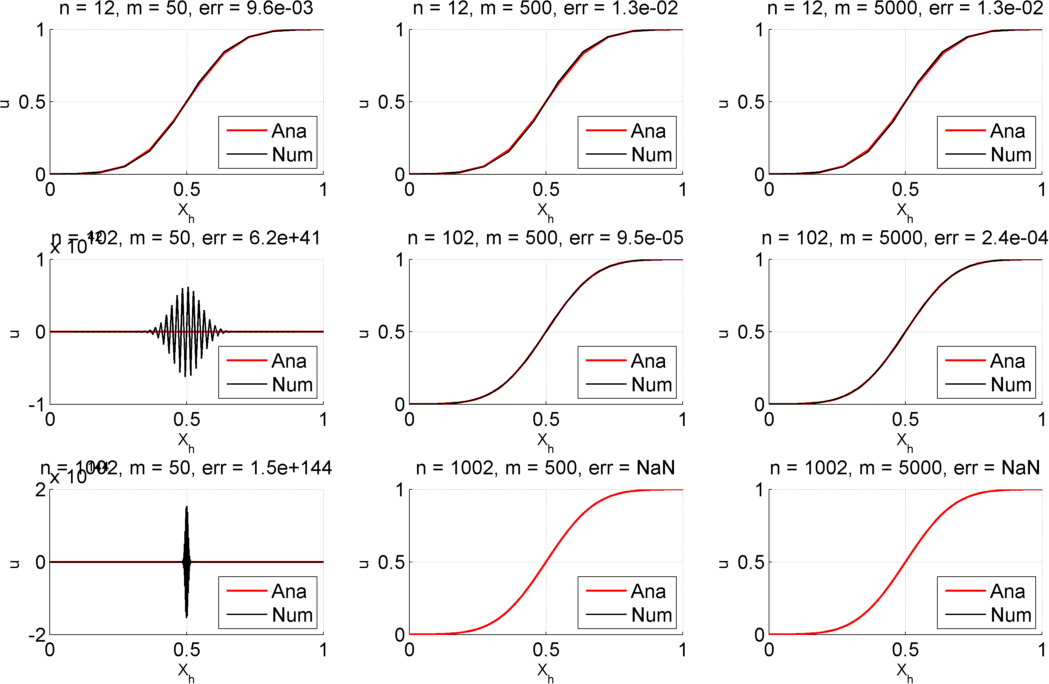
\includegraphics[width=0.96\textwidth]{a07ex01d_Theta1.png} 
	\caption{Solutions of the PDE for Euler Explicit Integration, $\Theta = 0$}
	\label{fig:a07ex01d_Theta1}
\end{figure}

\begin{figure}[H]
\vspace*{\FigUpperVSpace}
	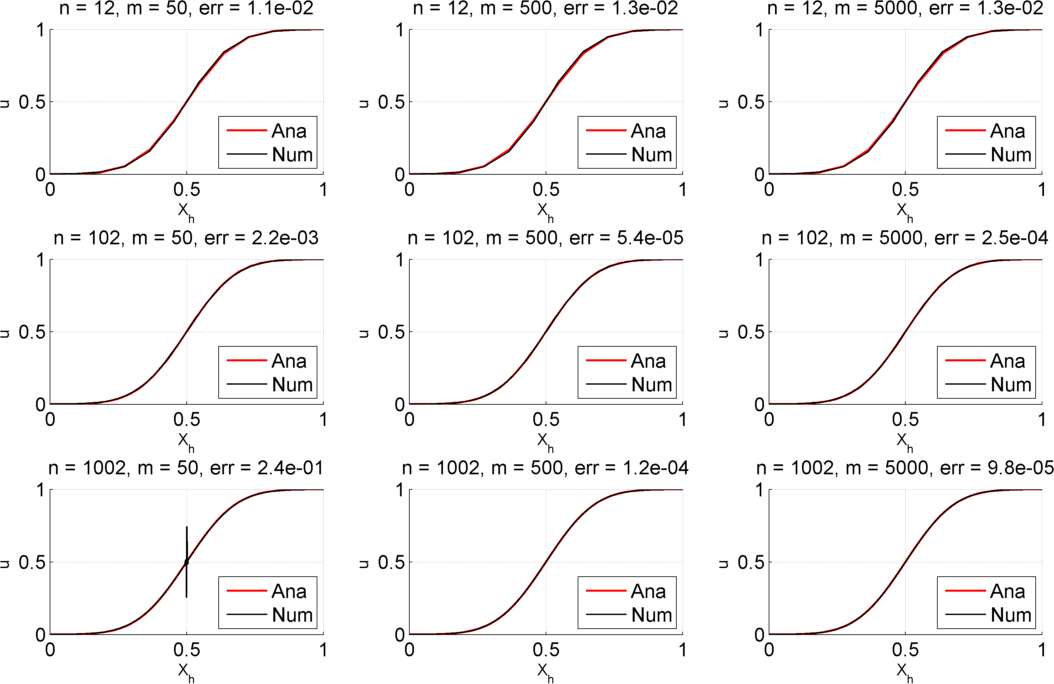
\includegraphics[width=0.96\textwidth]{a07ex01d_Theta2.png} 
	\caption{Solutions of the PDE be for Euler Implicit Integration, $\Theta = 1/2$}
	\label{fig:a07ex01d_Theta2}
\end{figure}
%
\vfill
%
\begin{figure}[H]
\vspace*{\FigUpperVSpace}
	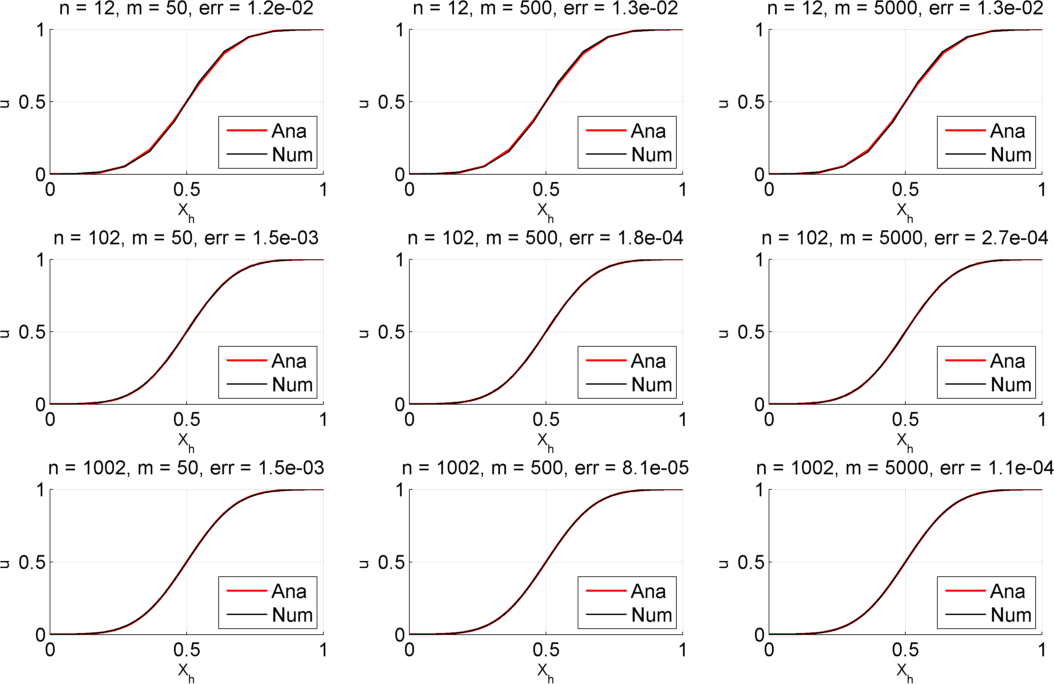
\includegraphics[width=0.96\textwidth]{a07ex01d_Theta3.png} 
	\caption{Solutions of the PDE be for Crank-Nicholson Integration, $\Theta = 1$}
	\label{fig:a07ex01d_Theta3}
\end{figure}
In the explicit Euler method (\FIG{a07ex01d_Theta1}), this requirement is violated for the $n=1002$ row, as well as for the solution from $n=102, m = 50$.
In contrast, the implicit Euler method (\FIG{a07ex01d_Theta3}) doesn't conflict with \EQ{stabReq}, as $\Theta = 0$ yields $1$ on the left hand side for every $M$ and $N$.
%
% ----------------
\addSubExercise{e}
With $\tau = \frac{T}{M}$, $M$ is also considerable in violating the stability in terms of \EQ{stabReq} requirement.
Results from d) show that Euler Explicit method may become rapidly hazardous, when $M$ is variated.
For Euler Implicit Method, the impact of vanishes.
Therefore, an arbitrary $M>0$ would satisfy the condition.
%
% ----------------
\addSubExercise{f}
In this exercise, the PDE with $u_0(x) = 0$, $f(x) = 1$, $g_0 = g_1 = 0$, $a = 1/100$, $b = 1$ and $T = 100$ was solved iteratively for three different $\Theta$ and for common difference stencils with $N = 50$ and $M=100$.
The solutions are plotted along with the analytical solutions in \FIG{a07ex01f} respectively.
In following these result are discussed.
For the implementation, please refer to online submitted \texttt{a07ex01f.m} files.
\begin{figure}[H]
\vspace*{\FigUpperVSpace}
	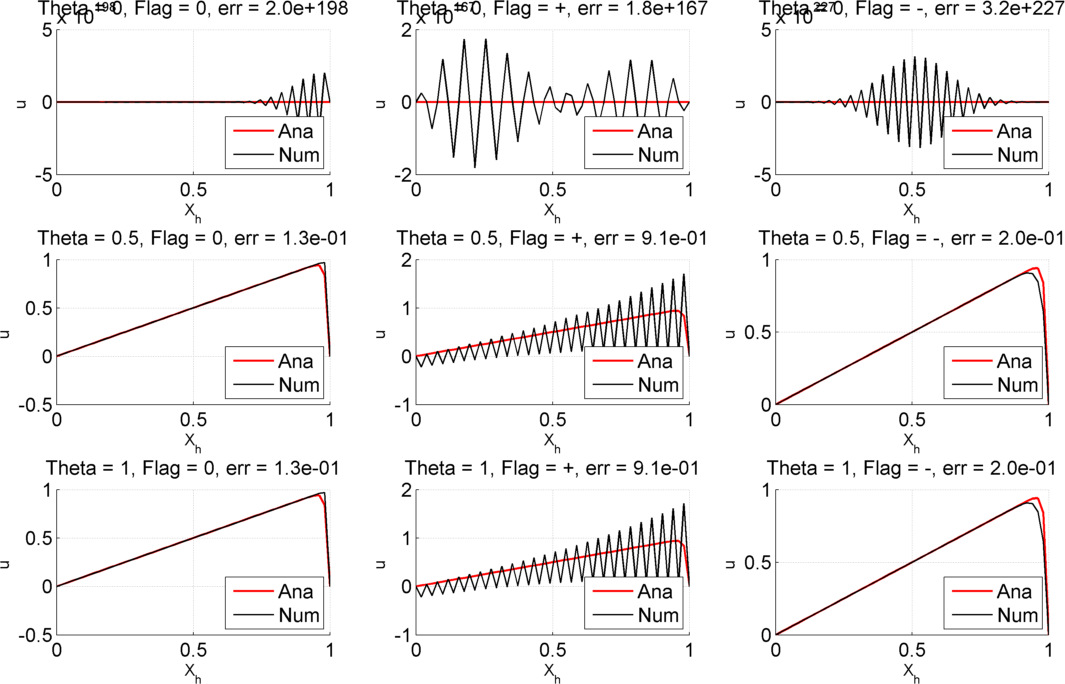
\includegraphics[width=0.96\textwidth]{a07ex01f.png} 
	\caption{Results of the Parabolic PDE for the considered integration methods, as well as difference stencils with $N$ = 50, $M = 100$.}
	\label{fig:a07ex01f}
\end{figure}
For $\Theta = 0$, all three solutions diverged due to not fulfilling the stability criteria in \EQ{stabReq}.
Furthermore, the forward difference stencil shows for $\Theta = 0.5$ and $\Theta = 1.0$ consistent results, if not converged.
\par
Running the simulation with $N = 200$ improves the convergence of the solutions in Euler Implicit and Crank-Nicolson methods for all three stencils, whereas the results from Euler Explicit method remains diverged.
%
% EXERCISE 2
% --------------------------------------------------------------------------------------------------------------------
\addExercise{2}{Ex02}

%
% ----------------
\addSubExercise{a}
Since the proposed function $u$ does not depend on t we have $\partial_t u = 0$ and so we have 
\begin{align*}
    -\Delta u &=-(\partial_{xx}+\partial_{yy}+\partial_{zz})u\\
			  &= (k^2\pi^2+l^2\pi^2+m^2\pi^2)u\\
			  &= \lambda_{klm}u\\
\end{align*}
%
which is an eigenfunction with eigenvalue 
%
\begin{equation*}
    \lambda_{klm}=\pi^2(k^2+l^2+m^2)
\end{equation*}
%
the normalization factor is given by
%
\begin{equation*}
    1=\int_0^1 u^2 dV 
	 = a_{klm}^2\int_0^1 sin(k\pi x)^2 dx \int_0^1 sin(l\pi y)^2 dy \int_0^1 sin(k\pi x)^2 dz\\
\end{equation*}
%
which for $k,l,m \in \mathbb{N}$ is
%
\begin{equation}
         a_{klm}= \sqrt{8}
\end{equation}
%
We can rewrite the inner product between $u_{klm}$ and $u_{nop}$ as
%
\begin{equation}
a_{klm}a_{nop}\int_0^1 sin(k\pi x)sin(n\pi x) dx \int_0^1 sin(l\pi y)sin(o\pi y) dy \int_0^1 sin(k\pi x)sin(p\pi x) dz
\end{equation}
%
The integral of the first term for $k$ with the corresponding normalization terms of $a_{klm}$ and $a_{nop}$ is of the form 
%
\begin{equation}
	sin(\pi k) cos(\pi n) - cos(\pi k) sin(\pi n)
\end{equation}
%
Which for $k,n \in \mathbb{N}$ is equal to $\delta_k^n$. We have a product of three of these kronecker deltas and obtain $\delta_{klm}^{nop}$ which is the definition of the function we wanted to show.
%
To show that the weights $w_{klm}$ are given by the equation
%
\begin{equation}
    \frac{1}{\lambda_{klm}} \int_\Omega f(x)u_{klm}(x)dxdydz
\end{equation}
%
we just substitute into $Lu=f$ and note that since $u_{klm}$ is a basis, we can also write $f(x)=\sum_{nop}w_{nop}u_{nop}$ as

\begin{align*}
    f=Lu =-\Delta u =-\Delta \sum_{klm} w_{klm} u_{klm} &= \sum_{klm} w_{klm} (-\Delta u_{klm})   \\
														&=\sum_{klm} \frac{1}{\lambda_{klm}} \int_\Omega f u_{klm} dxdydz (- \Delta u_{klm})\\
														&=\sum_{klm} \int_\Omega \left ( \sum_{nop}w_{nop}u_{nop}\right ) u_{klm} dxdydz \cdot u_{klm} \\
														&=\sum_{klm} \left ( \sum_{nop}   \int_\Omega  w_{nop}u_{nop} u_{klm} dxdydz \right ) \cdot u_{klm} \\
														&=\sum_{klm} \left ( \sum_{nop}   w_{nop} \int_\Omega  u_{nop} u_{klm} dxdydz \right ) \cdot u_{klm} \\
\text{.}
\end{align*}
%
Given that $ \int_\Omega  u_{nop} u_{klm} dxdydz =\delta_{klm}^{nop}$ this cancels out the inner sum, so we have:
%
\begin{align*}
    f=Lu =\sum_{klm} w_{klm} \cdot u_{klm}
\end{align*}
%
For $f=1$ we have 
%
\begin{align*}
    w_{klm}&=\frac{1}{\lambda_{klm}} \int_\Omega u_{klm} dxdydz\\
		   &=\frac{a_{klm}}{\lambda_{klm}}  \int_0^1 sin(k\pi x) dx \int_0^1 sin(l\pi y) dy \int_0^1 sin(k\pi x) dz\\
		   &=\frac{a_{klm}}{\lambda_{klm}}  \frac{8}{\pi^3klm}\\
\end{align*}
%
which since $k,l,m \in \mathbb{N}$ reduces to:
%
\begin{equation}
	w_{klm}=
	\begin{cases}
	\frac{a_{klm}}{\lambda_{klm}}  \frac{8}{\pi^3klm}, & \text{if}\ k,l,m \text{ all divisible by 2} \\
	0, & \text{otherwise}
	\end{cases}
\end{equation}
%
% ----------------
\addSubExercise{b}
In this exercise, the sample code from assignment 4 was extended to $\Omega = (0,1)^3$ and the problem $-\Delta u = 1$ was solved with homogeneous Dirichlet boundary conditions.
\FIG{heatb} illustrates the solution, whereas the error is plotted in \FIG{error2b}.
For the implementation, please refer to the online submitted \texttt{a07ex02b.py} file.
%
% ----------------
\addSubExercise{c}
Please refer to the online submitted \texttt{a07ex02c.py} file.
%
% ----------------
\addSubExercise{d}
The error is plotted in \FIG{error_d}.
Please refer to the online submitted \texttt{a07ex02d.py} and \texttt{a07ex02d\_error.py} files.

% FIGURES
% ---------------------------------------------
\begin{figure}[H]
	\centering
	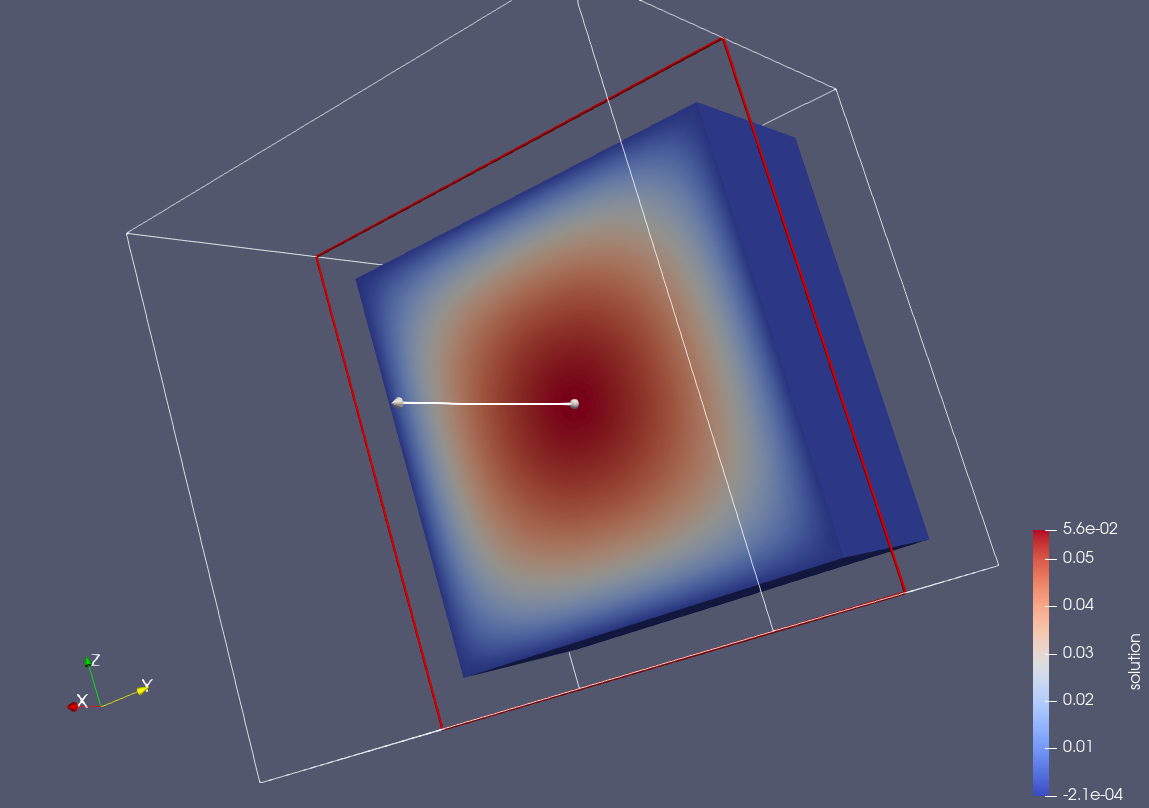
\includegraphics[width=\textwidth]{heatb.png} 
	\caption{Solution from 2a, very similar as 2b}
	\label{fig:heatb}
\end{figure}
\vfill
\begin{figure}[H]
	\centering
	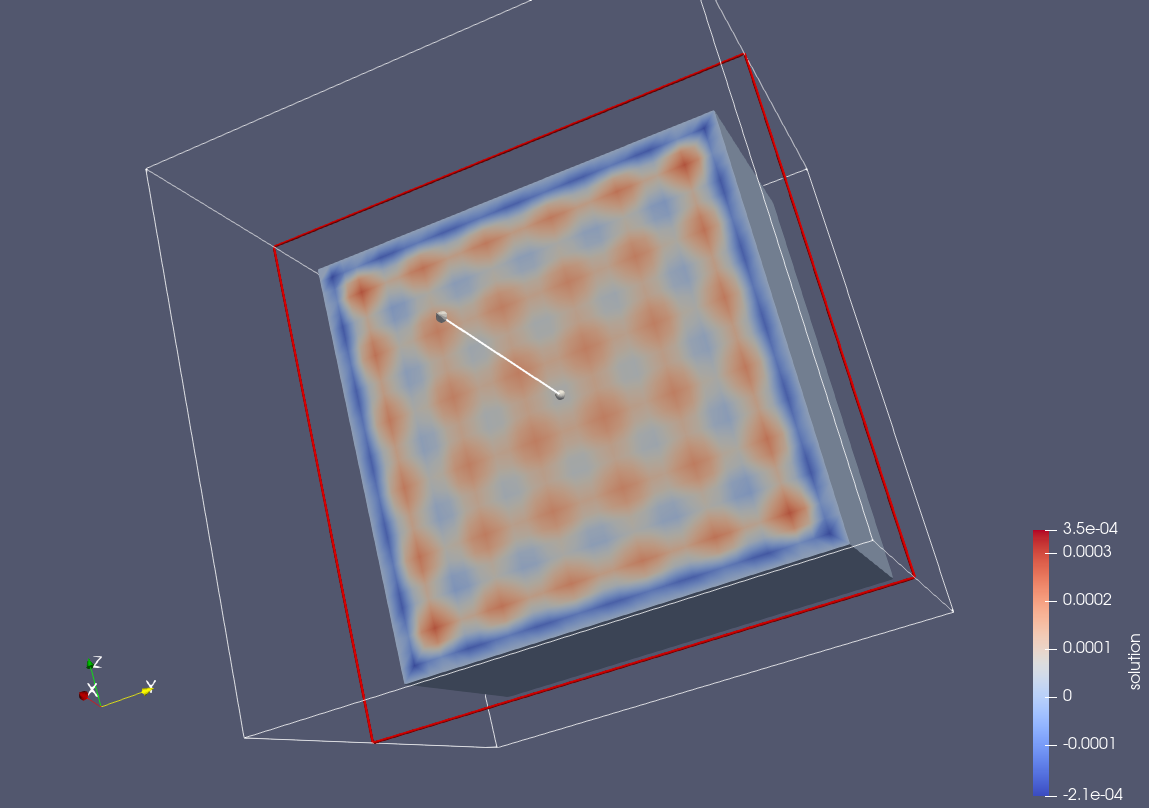
\includegraphics[width=\textwidth]{error2b.png} 
	\caption{Error between 2a an 2b. Note that the relative error is of about two orders of magnitude.}
	\label{fig:error2b}
\end{figure}

\begin{figure}[H]
	\centering
	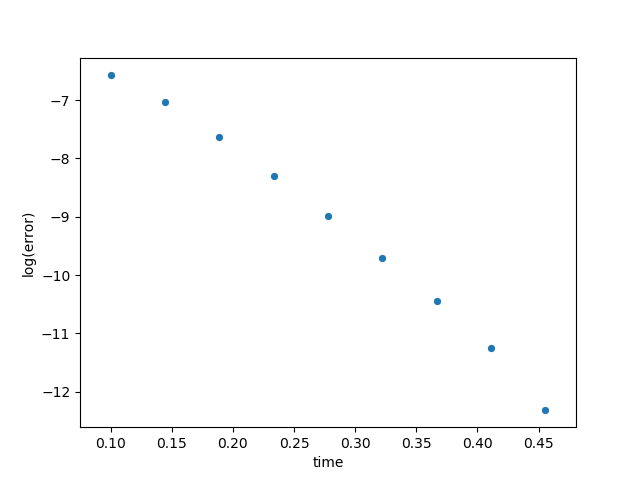
\includegraphics[width=\textwidth]{error_d.png} 
	\caption{Error between the exact solution and the one computed numerically using the implicit Euler method. Note that even though the error decreases, it stabilizes around a value of 0.000709, which was subtracted in order to better distinguish a possibly stable decreasing error rate }
	\label{fig:error_d}
\end{figure}